\section{Interaction and Teaching Capabilities}
\label{sec:teaching}

To quickly adapt our robot to new store environments and products, we created four interfaces for operators: a digital twin for remote monitoring and control,adding product classes to the perception, trajectory teaching mode, and audio explanations of the robot's skills. 

\subsection{Digital Twin for Remote Monitoring and Control}
\label{sec:digital_twin}

\begin{figure*}[t]
  \begin{center}
    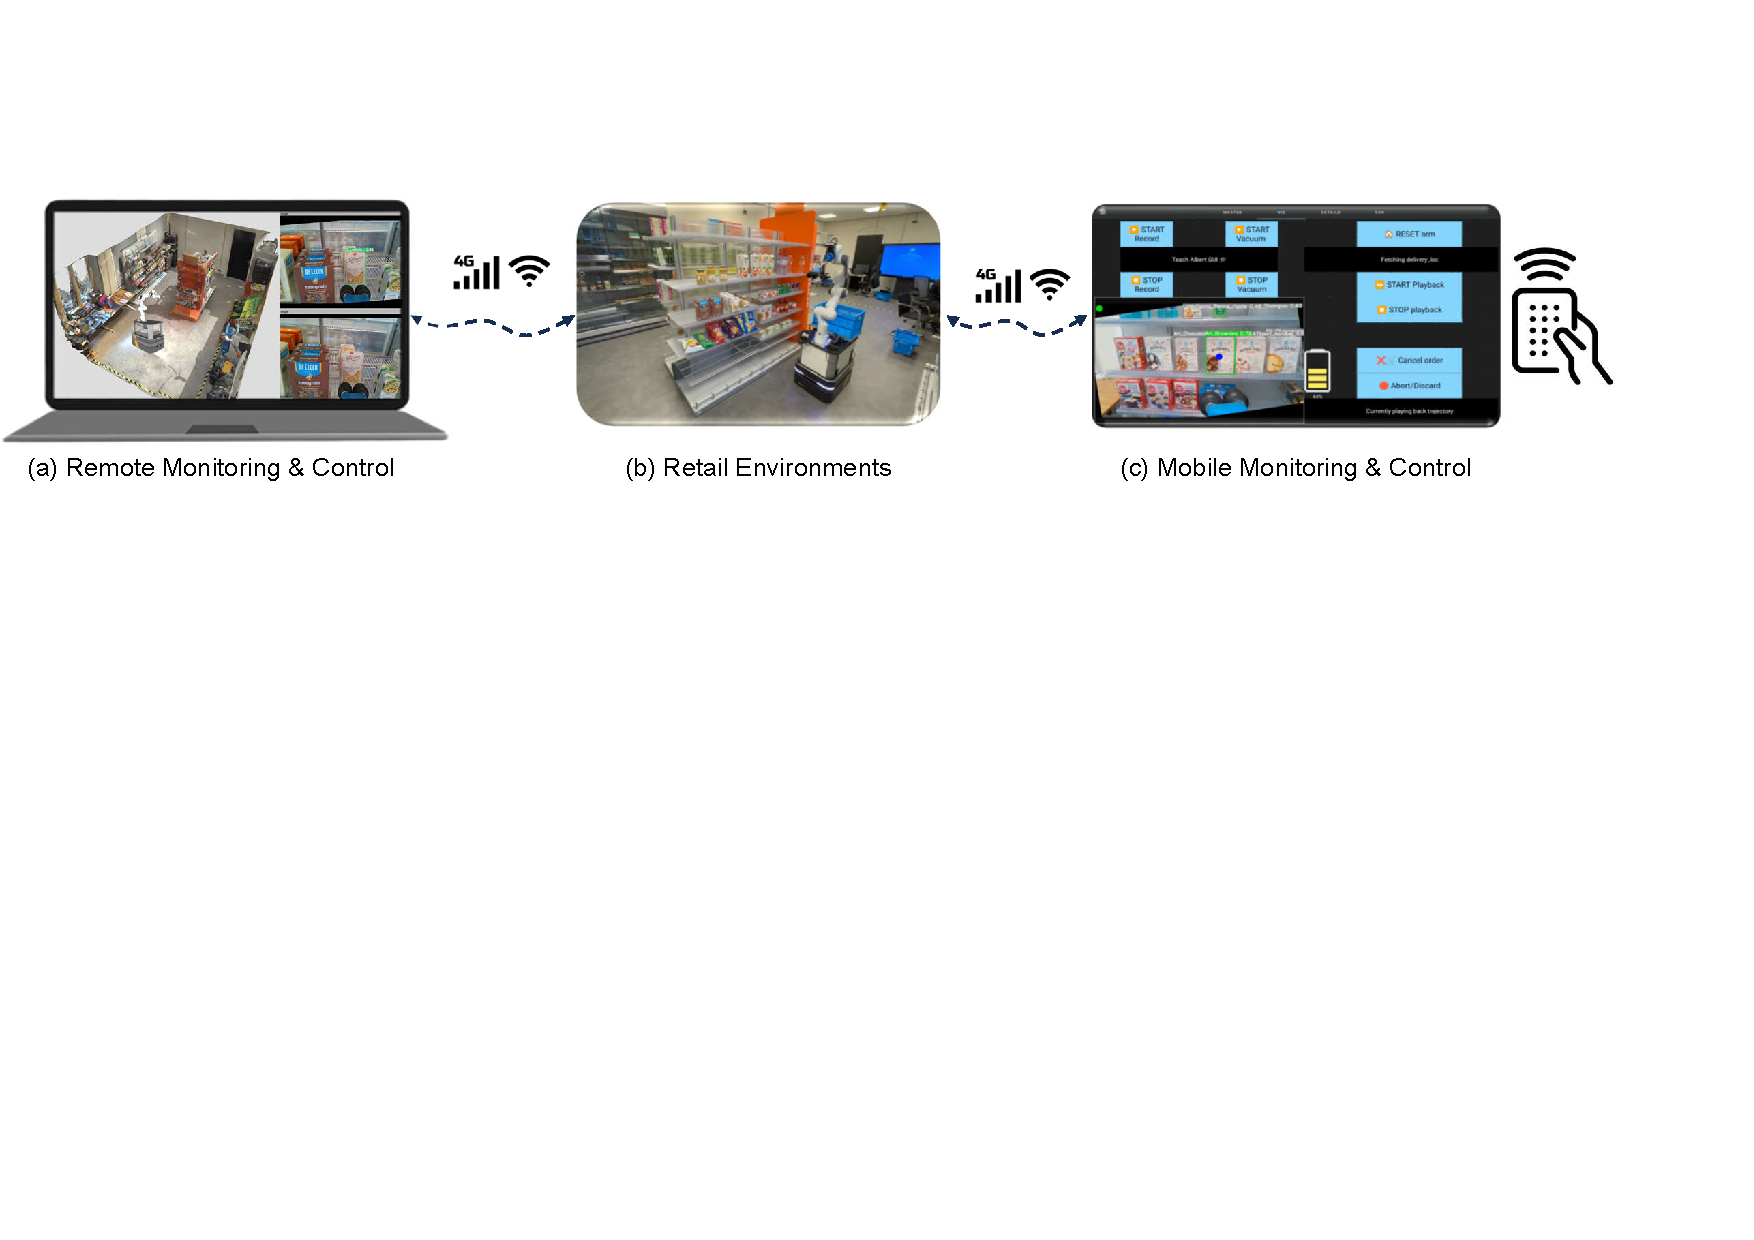
\includegraphics[width=0.85\linewidth]{remote_v5.pdf}
  \end{center}
  \caption{Overview of the remote monitoring and control system. a) Laptop-based remote interface for monitoring and control system; b) Visualization of the robot within the actual retail environment; c) Tablet interface for on-the-go monitoring and task programming}\label{fig:remote_overview}
\end{figure*}

Herein, we introduce a digital twin mechanism to support remote monitoring and control of a mobile manipulator in a retail setting, as shown in Fig.~\ref{fig:remote_overview}. By scanning the environment in three dimensions, we construct a virtual model that accurately represents the workspace. The robot, when operational in a supermarket, is connected to this digital twin through Wi-Fi or 4G, enabling operators to monitor its status and issue commands from any remote location. The addition of a tablet interface allows for flexible monitoring and control by on-site staff, who can easily adjust the robot's course or teach it new tasks as needed.




\begin{figure}[t]
  \centering
  \begin{subfigure}[b]{0.45\linewidth}
    \centering
    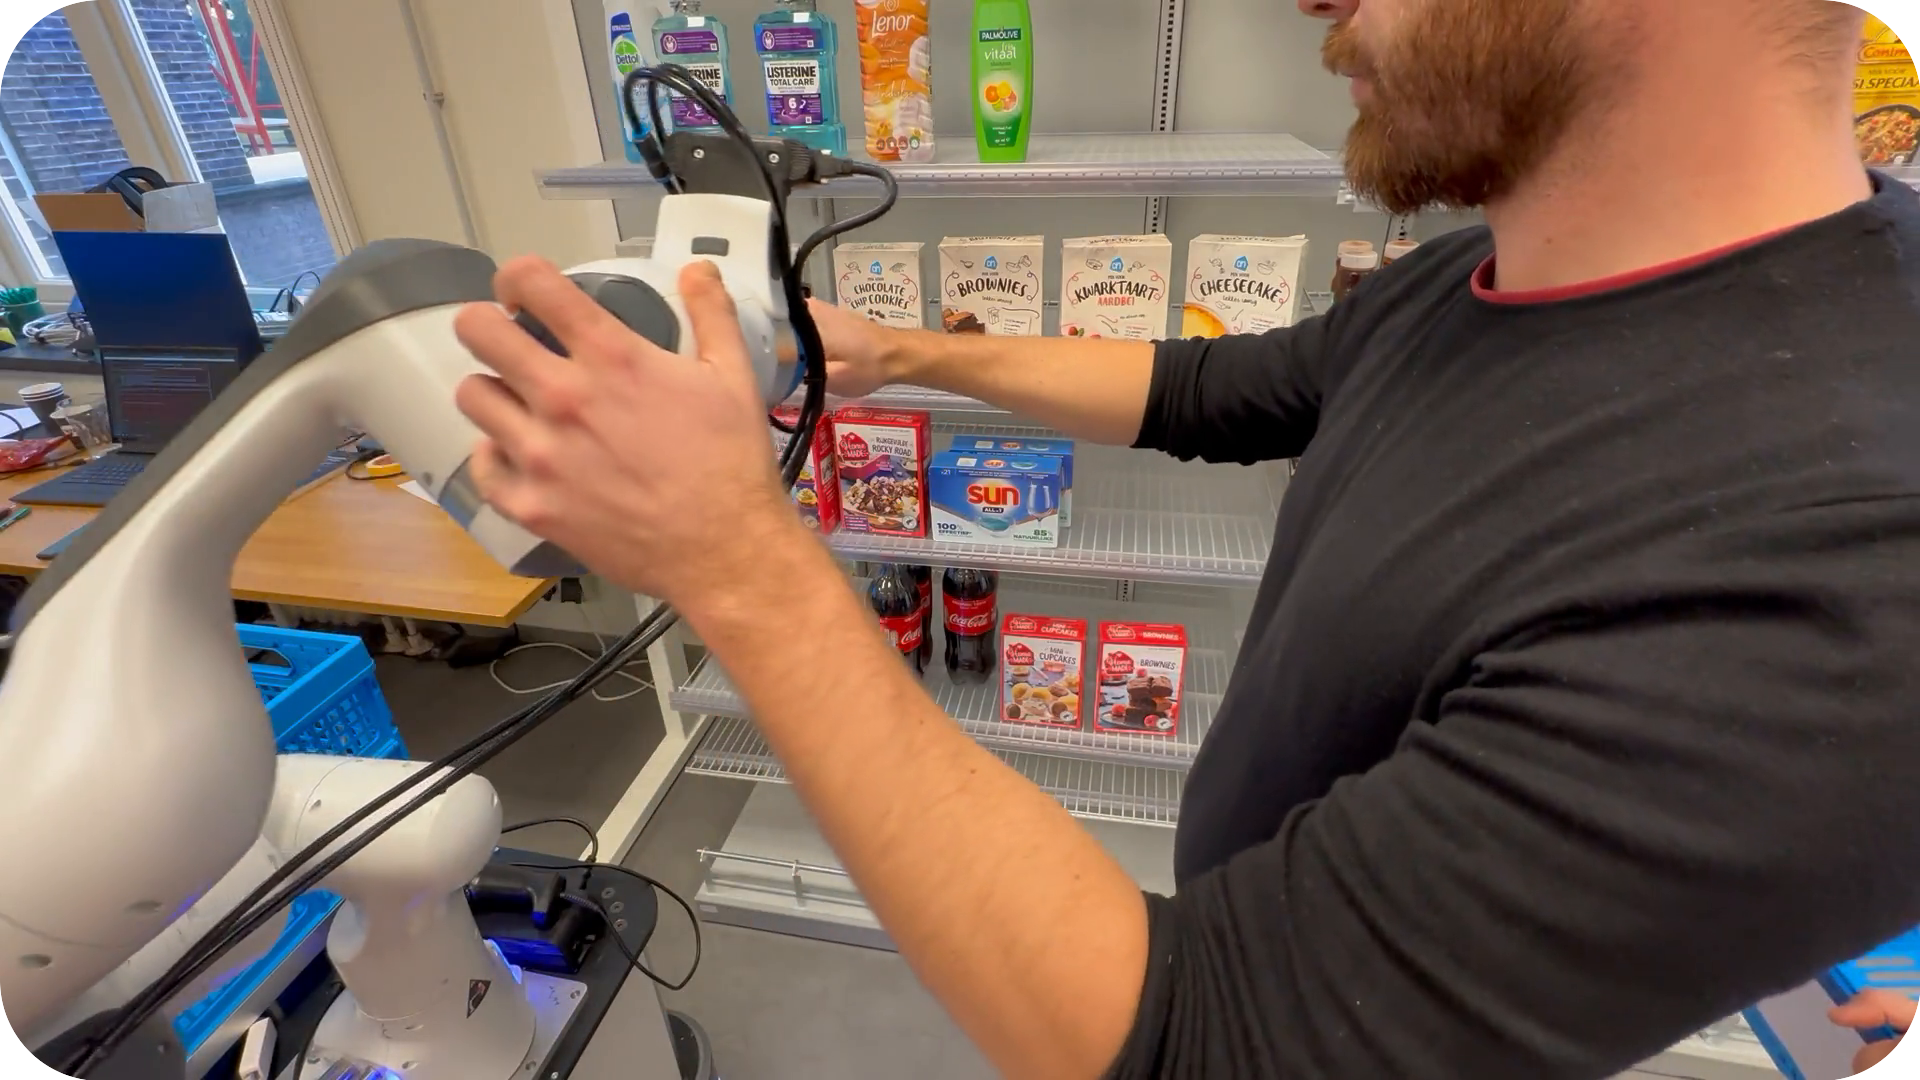
\includegraphics[width=0.95\textwidth]{teaching_005_rounded.png}
    \caption{}
    \label{subfig:teaching_1}
  \end{subfigure}
  \begin{subfigure}[b]{0.45\linewidth}
    \centering
    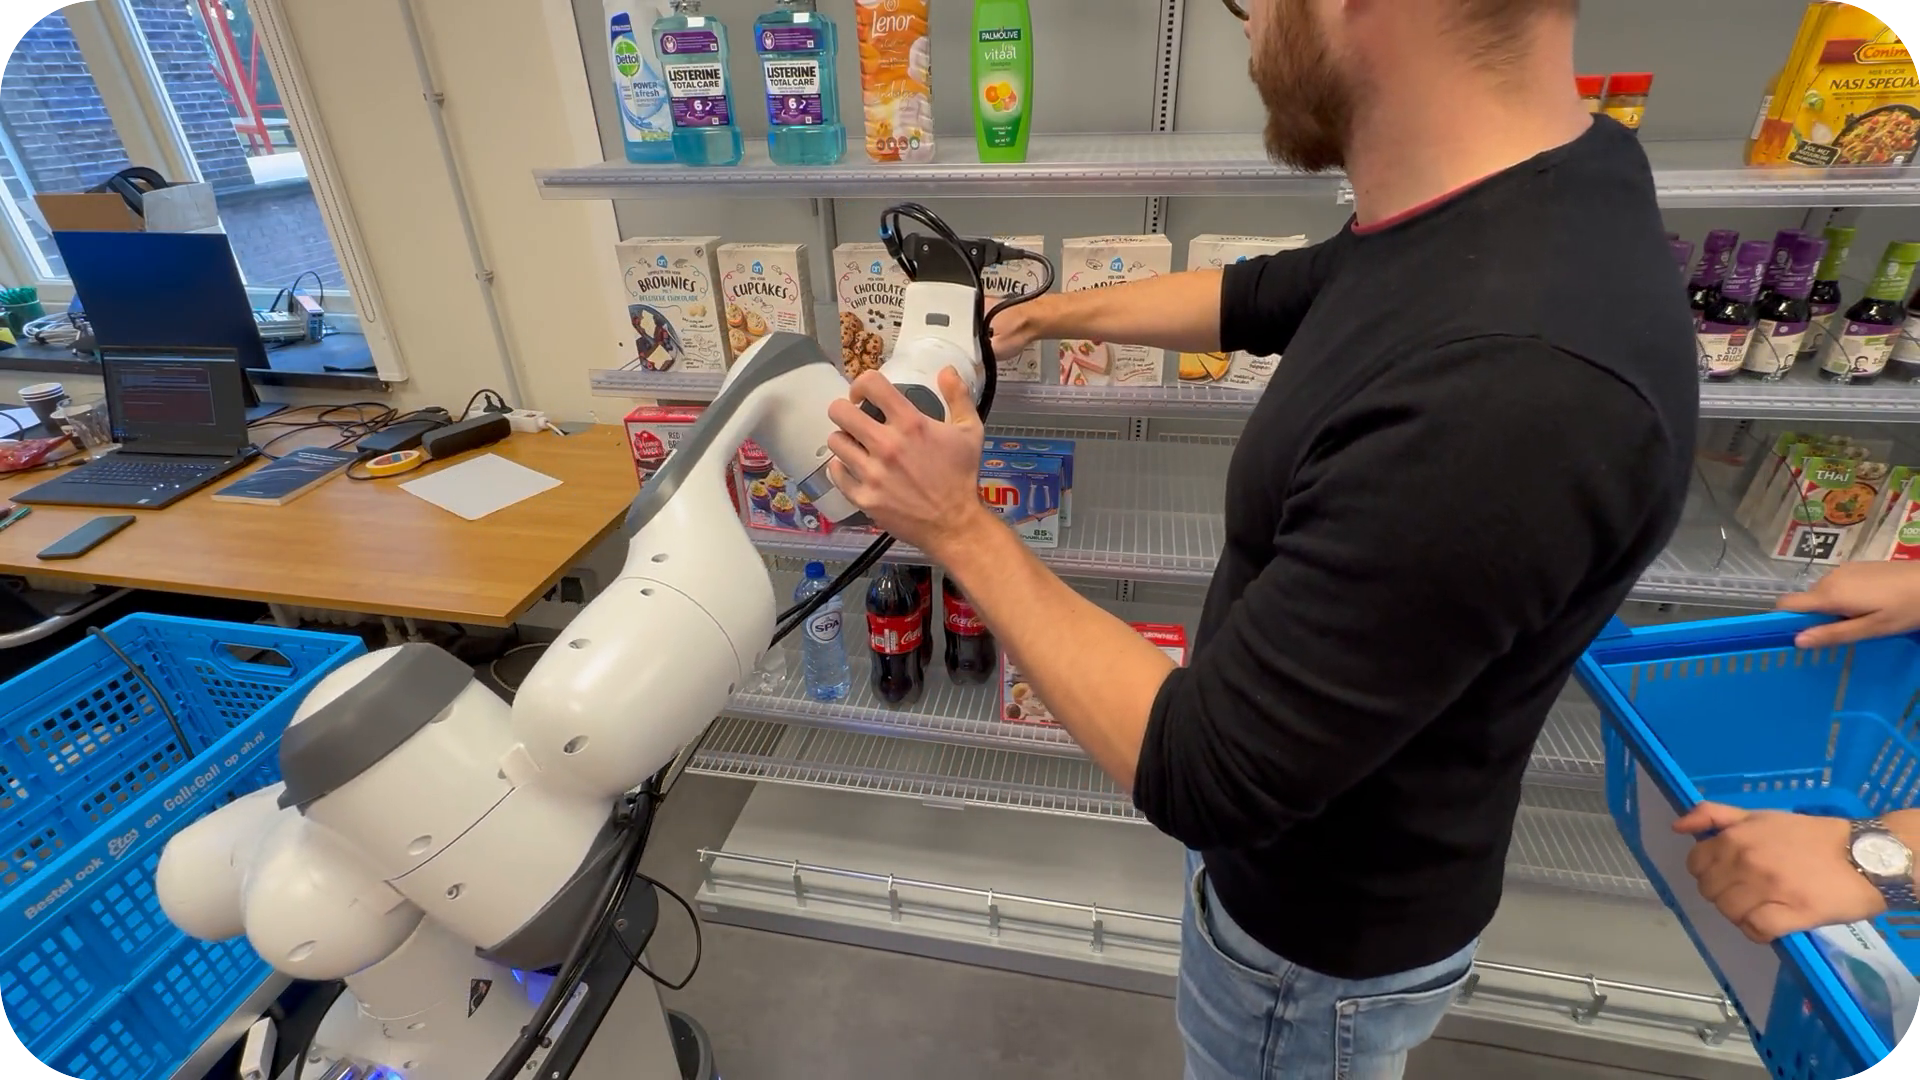
\includegraphics[width=0.95\textwidth]{teaching_009_rounded.png}
    \caption{}
    \label{subfig:teaching_2}
  \end{subfigure}
  \begin{subfigure}[b]{0.45\linewidth}
    \centering
    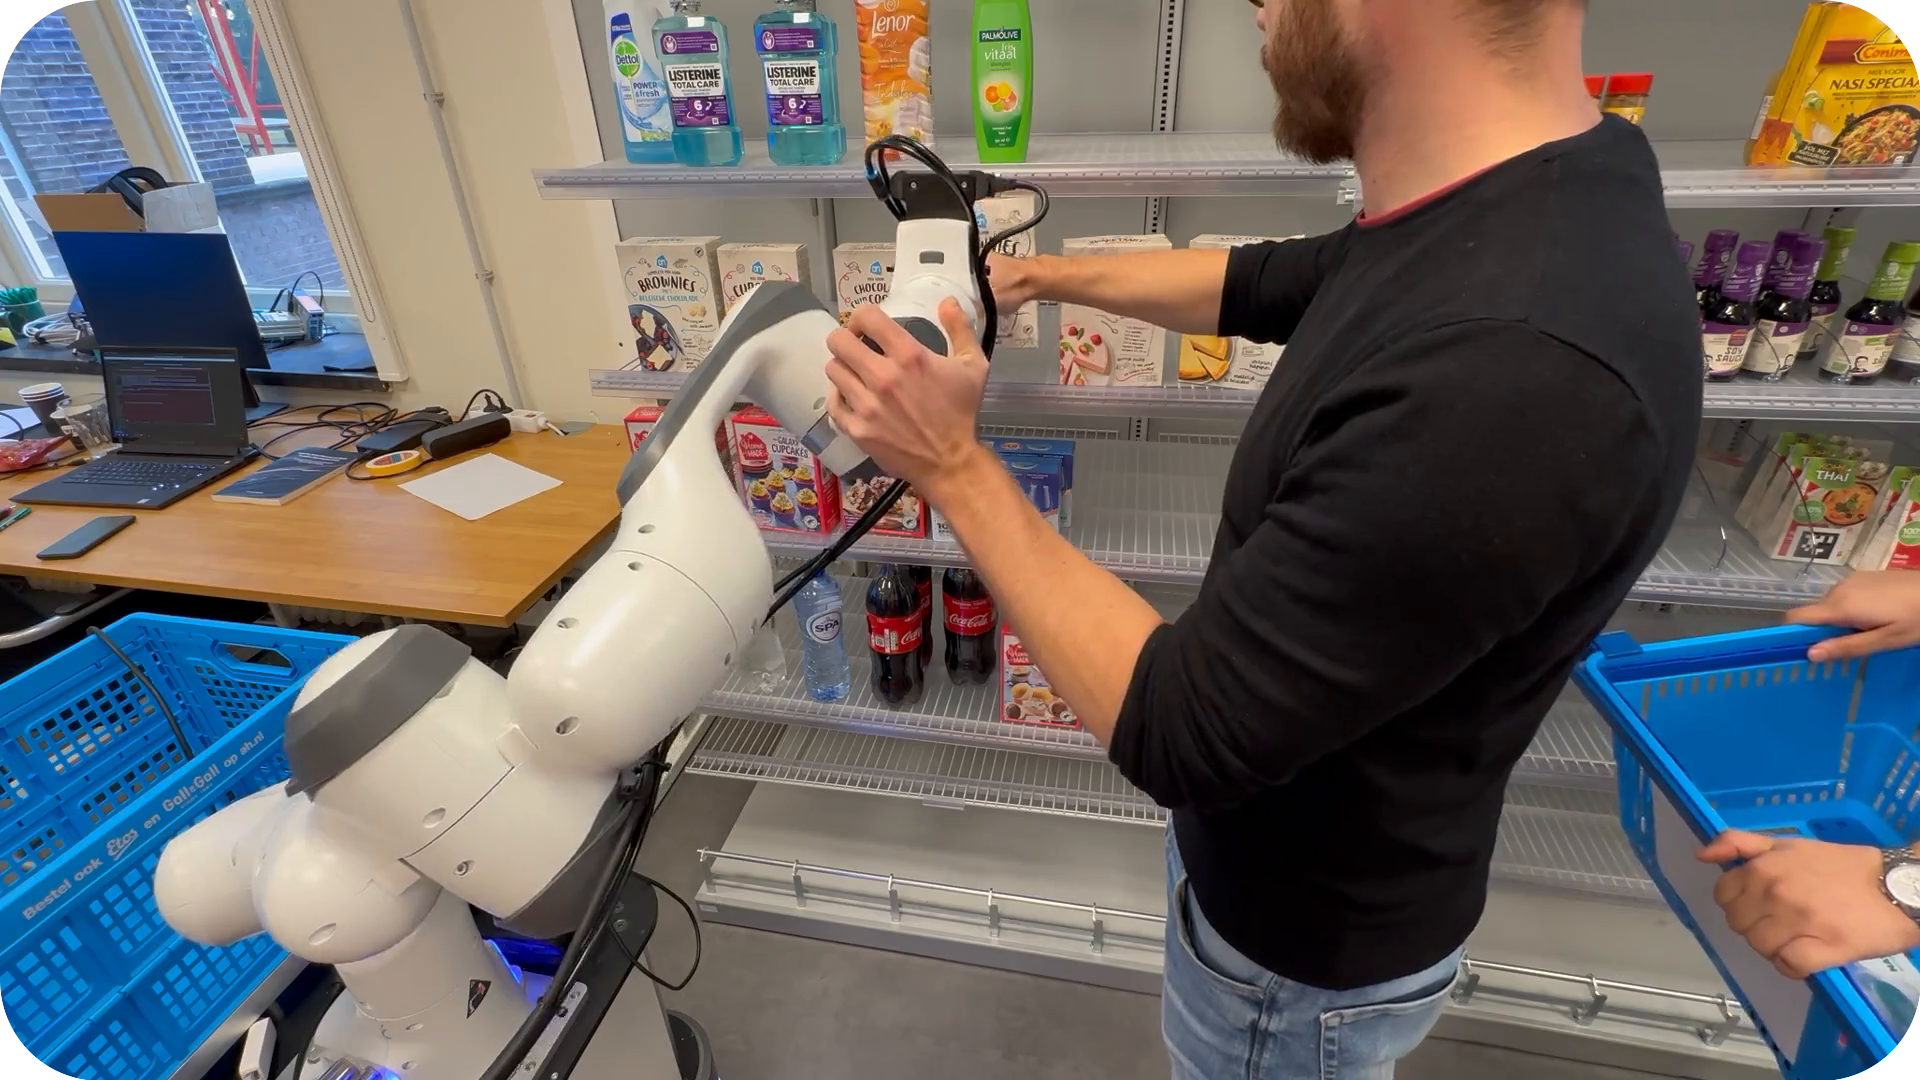
\includegraphics[width=0.95\textwidth]{teaching_011_rounded.png}
    \caption{}
    \label{subfig:teaching_3}
  \end{subfigure}
  \begin{subfigure}[b]{0.45\linewidth}
    \centering
    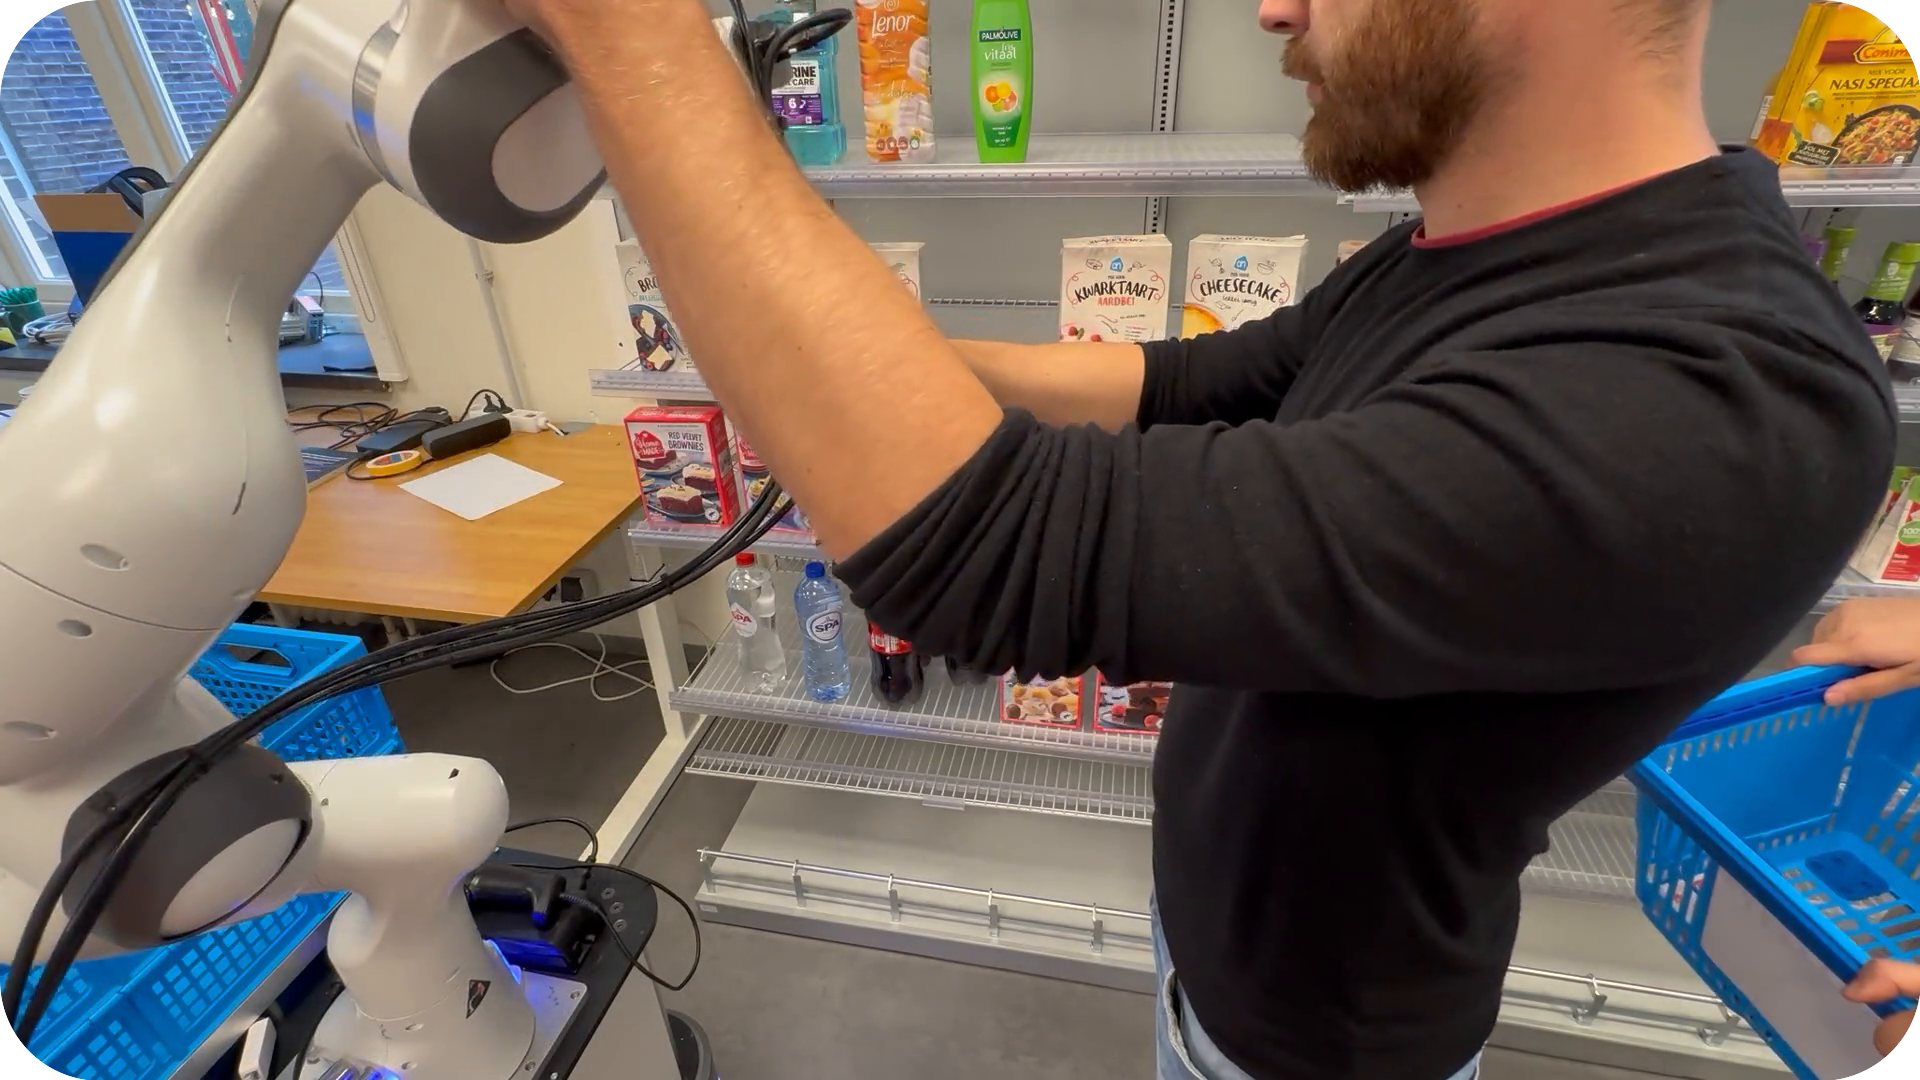
\includegraphics[width=0.95\textwidth]{teaching_014_rounded.png}
    \caption{}
    \label{subfig:teaching_4}
  \end{subfigure}
  \caption{The human operator can easily `teach' the robot a new picking
  strategy by moving the arm, thus passing implicit knowledge to the
  robot.}
  \label{fig:recording}
\end{figure}
\subsection{Interactively adding product classes to perception}
Sec.~\ref{sec:perception} explains ProtoProductNet, our adaptation to the state-of-the-art ProtoNet, to make the few-shot learning approach scalable for the supermarket environment. To add new unseen product classes to ProtoProductNet, we developed a custom user interaction for human operators. The interaction contains the following steps 1) the operator uses a barcode scanner, attached to the robot, to scan the new product 2) the operator puts the product in view in front of the robots camera 3) a GUI with the view of the camera pops up on the screen and the operator interactively drags a box around the new product. The robot should already start detecting the product, as can be verified by a bounding box appearing on screen. To further enhance the detection the operator can add images from different angles of the product. The cropped images selected by the operator are saved locally and combined with the product's barcode. If the same barcode is encountered in future orders, our perception pipeline will now know how to classify the product accurately, without retraining the network.

\subsection{Teaching grasping trajectories to the robot}
\label{sub:teaching}

As explained in Sec.~\ref{sec:trajectory_generation}, \ac{fabrics} require global guidance to effectively execute complex actions.
To simplify the process of obtaining this guidance in the form of trajectories, we leverage human expert demonstrations, effectively teaching the robot.
We distinguish between two
phases for teaching, the \textit{recording} and the
\textit{playback}. For both phases, we assume that the product
is visible and detected by the robot, such that we can
compute a transformation between the root link and the product.

\subsubsection{Recording}
When recording a trajectory, we first reduce the stiffness
of the robot to the bare minimum, such that it can easily be
pushed around by the human operator. Then, the human
operator can activate recording by pressing a button on our tablet interface. From that moment onwards, the state values \x{} for the
constraints defined for picking in Sec.~\cref{sub:picking}
are recorded, see \cref{fig:recording}.
The state of the gripper, active
or non-active, and whether a product is attached to the gripper
are also recorded.
%For the sake of memory efficiency, we
%ignore trajectory points if they are too similar to the
%previous one.
We additionally record the
transformation matrix between the root link of our kinematic
chain and the product to be picked. That allows us to later
generalize the recording to different product poses by applying a rigid body transformation to the trajectory.


\subsubsection{Playback}

During trajectory playback, we loop through the recorded goals sequentially, continuing when a desired goal accuracy has been reached. 
%When playing back a trajectory, the trajectory points are
%passed to the trajectory generator as goals in a sequential
%manner. Proceeding to the subsequent trajectory point
%requires that the current one has been reached up to a
%desired accuracy. 
In contrast to the recording part, where
we exclude motion of the base, during playback the base motion is activated, see \cref{fig:base_motion}.
To account for different product poses
between recording and playback, we transform the goals on the fly based on the product pose estimate, see Sec.~\ref{sec:perception}, using the following transform:
\[
  _{\product,r}\mat{T}^{\product,p} =
  \left(_{0}\mat{T}^{\product,r}\right)^{-1}_{0}\mat{T}^{\product,p}.
\]
Using this continual feedback we effectively employ a visual servoing \cite{kmich2022image} approach and are robust against changes in product location during the pick.
In addition to \ac{fabrics} goals, the recording also contains information about the state of the vacuum pump. This state information is replicated during playback, and used to know when a product should have been attached.
In the playback routine of the picking action we then modify the fabrics goal if a product is not yet attached where it is expected. The goal is modified to effectively push further into the shelf along the z-axis of the nozzle head, until a product is attached, or a maximum threshold is reached.
\begin{figure*}[t]
  \centering
  \begin{subfigure}[b]{0.20\linewidth}
    \centering
    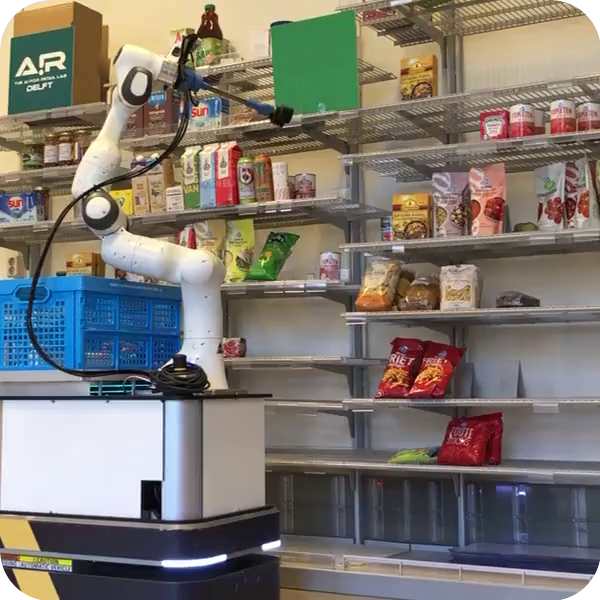
\includegraphics[width=0.95\textwidth]{base_motion_002_rounded_wo.png}
    \caption{}
    \label{subfig:base_motion_1}
  \end{subfigure}
  \begin{subfigure}[b]{0.20\linewidth}
    \centering
    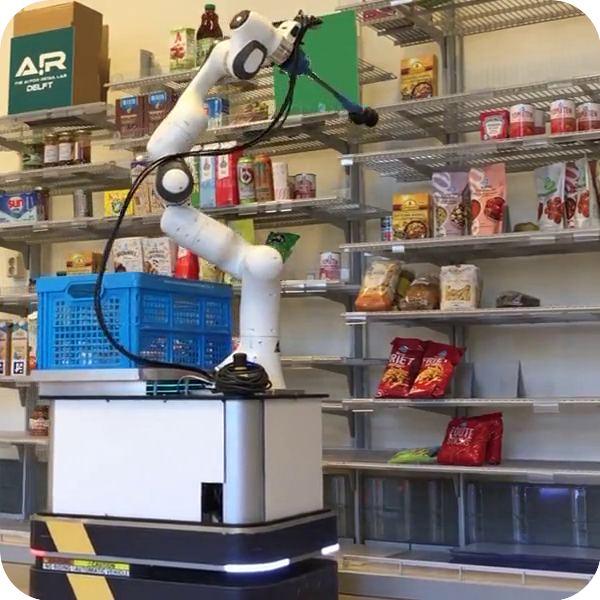
\includegraphics[width=0.95\textwidth]{base_motion_003_rounded_wo.png}
    \caption{}
    \label{subfig:base_motion_2}
  \end{subfigure}
  \begin{subfigure}[b]{0.20\linewidth}
    \centering
    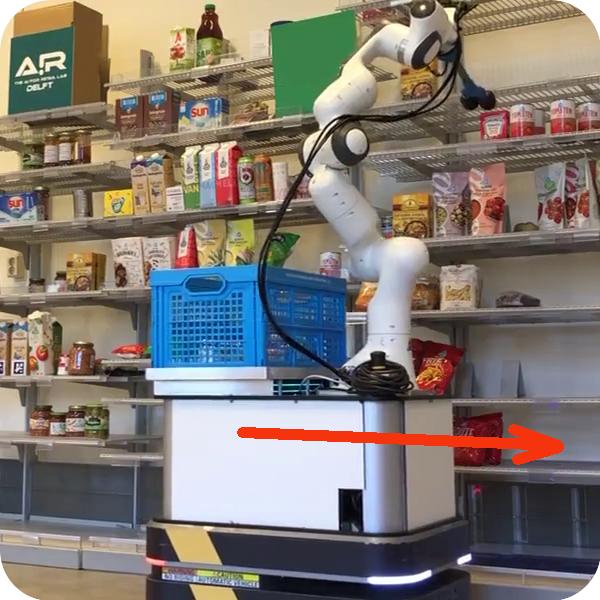
\includegraphics[width=0.95\textwidth]{base_motion_004_rounded_wo.png}
    \caption{}
    \label{subfig:base_motion_3}
  \end{subfigure}
  \begin{subfigure}[b]{0.20\linewidth}
    \centering
    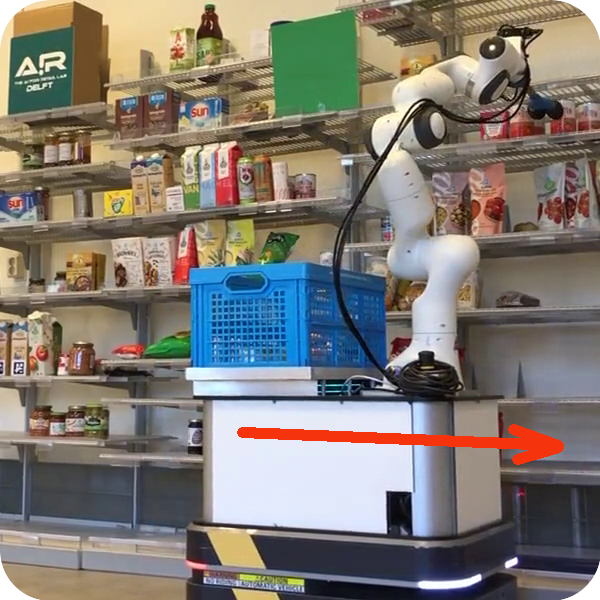
\includegraphics[width=0.95\textwidth]{base_motion_005_rounded_wo.png}
    \caption{}
    \label{subfig:base_motion_4}
  \end{subfigure}
  \caption{During playback, \ac{fabrics}  actively use the base's forward motion as a prismatic joint to compensate for misplacement during navigation.}
  \label{fig:base_motion}
\end{figure*}

\subsection{Audio feedback}
\label{sec:language_feedback}

During the robot's operation, we are interested in providing audio explanations of the robot's actions as feedback to operators, e.g., to monitor the robot and to be notified about failures. 
We do this by 1) generating compact prompts of the robot's action and state and 2) using Large Language Models (LLMs) to generate short informative explanations that are played via the robot's speaker.


\paragraph{Prompt generation}
We leverage the structure of the generated behavior trees and symbolic state information (see Sec.~\ref{sec:decision_making}) to generate prompts for an LLM. 
For every sub-tree in the generated Behavior Tree, we automatically add action nodes that generate prompts for actions and items.
An action is described by its name $a$ formulated as a verb in the present continuous form, e.g., $a=\texttt{placing}$.
The item's name $i$ is taken from the product database, e.g., $i=\textit{Whole Milk}$.
We generate string prompts of the form $pr$:
\begin{equation*}
    pr := \textit{action }~a~i~c,
\end{equation*}
where $c\in\{\texttt{running},\texttt{failed}, \texttt{completed}, \texttt{retry}\}$ is the status returned from the sub-tree.
An example for a generated prompt is ``\textit{action }\texttt{picking }\texttt{Whole Milk }\texttt{retry}''.


\paragraph{Explanation generation}
We generate explanations by prompting an LLM on the fly with our generated prompts. 
To this end, we provide the LLM with a context describing that the robot is deployed as an order picking robot in a supermarket with five skills and that the task is to generate a concise explanation of the prompt to operators. 
During operation of the robot, we simultaneously generate the explanations and play them back via the robot's speaker.
For instance, for the prompt  ``\textit{action }\texttt{picking }\texttt{Whole Milk }\texttt{retry}'', we generate the explanation: ``Oops! It seems like I had a little trouble placing the Whole Milk into my basket. No worries, I'll give it another
  try and make sure it goes in smoothly this time''.

